\documentclass[conference]{IEEEtran}
\IEEEoverridecommandlockouts
\usepackage{cite}
\usepackage{amsmath,amssymb,amsfonts}
\usepackage{newtxtext,newtxmath}
\usepackage{booktabs}
\usepackage{tabularx}
\usepackage{array}
\usepackage{listings}
\usepackage{xcolor}
\usepackage{tikz}
\usetikzlibrary{arrows.meta,positioning}
\usepackage[hidelinks]{hyperref}
\usepackage{url}
\usepackage{flafter}
\usepackage{float}
\usepackage{needspace}
\usepackage{balance}
\setcounter{dbltopnumber}{5}
\setcounter{totalnumber}{6}
\renewcommand{\dbltopfraction}{0.95}
\renewcommand{\dblfloatpagefraction}{0.85}
\setlength{\textfloatsep}{8pt plus 2pt minus 2pt}
\lstset{basicstyle=\ttfamily\scriptsize,breaklines=true,columns=fullflexible,keepspaces=true,frame=single,framerule=0.2pt,xleftmargin=2pt,xrightmargin=2pt,aboveskip=4pt,belowskip=4pt}
\clubpenalties 3 10000 10000 0
\hypersetup{pdftitle={SPIRA Submission B},pdfauthor={Jeewon Lee, Uijin Lee, Seojin Lee, Yejoon Kim}}
\title{SPIRA: Proactively Preparing Smart Homes via Retrieval-Augmented Purchase Intent Inference over Synthetic Knowledge}
\author{
\IEEEauthorblockN{Jeewon Lee}
\IEEEauthorblockA{\small\textit{Dept. of Information Systems}\\\textit{Hanyang University}\\Seoul, Republic of Korea\\leejeewon916@gmail.com}
\and
\IEEEauthorblockN{Uijin Lee}
\IEEEauthorblockA{\small\textit{Dept. of Information Systems}\\\textit{Dept. of Food \& Nutrition}\\\textit{Hanyang University}\\Seoul, Republic of Korea\\smilelejn@gmail.com}
\and
\IEEEauthorblockN{Seojin Lee}
\IEEEauthorblockA{\small\textit{Dept. of Information Systems}\\\textit{Hanyang University}\\Seoul, Republic of Korea\\leeseojini0303@gmail.com}
\and
\IEEEauthorblockN{Yejoon Kim}
\IEEEauthorblockA{\small\textit{Dept. of Information Systems}\\\textit{Hanyang University}\\Seoul, Republic of Korea\\yejoonkim1340@gmail.com}
}
\IEEEaftertitletext{\vspace{-\baselineskip}{\centering\footnotesize CSE 406 Software Engineering --- Team SPIRA --- Submission B\par}\vspace{0.5em}}
\begin{document}
\maketitle
\raggedbottom
\begin{abstract}
Online delivery brings products to the door, but users must still prepare the home for the situation those products may indicate. We propose \textbf{SPIRA}, which connects a shared order to household preparation through retrieval-augmented purchase-intent inference. Synthetic purchase-intent cases provide cold-start knowledge for a one-shot interpretation of the order and its relevant time or calendar context. A deterministic gate and plan validation constrain the resulting household tasks. SPIRA announces the preparation through a notification with stop, per-task disable, and explanation controls. Local execution checks current capability and physical state, observes command outcomes, and respects user intervention. Household memory links the inferred situation to attempted work, actual results, and explicit reactions. The initial prototype targets a child's birthday party with clearly labeled physical and simulated devices. The following sections update the submitted requirements and specify the development environment and end-to-end process.

\end{abstract}
\begin{IEEEkeywords}smart home, purchase intent, synthetic knowledge, retrieval-augmented inference, household preparation\end{IEEEkeywords}
\section{Introduction}
\subsection{Motivation}
A delivery service brings products to the door. Household preparation still requires the user's effort. After an order arrives, the user must decide how each item should be stored, treated, or used. The same strawberry should be handled differently when it is an ordinary grocery item and when it is intended for decorating cupcakes at a birthday party. Perishable ingredients may also require care before the occasion. These decisions are small individually, but they accumulate at the exact time when online shopping is supposed to reduce effort.

A second burden appears when several purchased items indicate a future occasion. Buying party decorations, children's tableware, cupcake ingredients, and drinks can support an interpretation of a household situation. Users must translate that situation into separate actions such as cleaning before guests arrive, preparing child-safety settings, changing lighting and media, and placing an oven in a ready state. Existing smart-home routines can automate these actions only after the user has already recognized the situation and configured the corresponding rules. SPIRA connects purchase-intent evidence to situation-driven home preparation. Bounded item-handling guidance and loss prevention remain supporting responsibilities, including for an item outside a special-occasion bundle.

\subsection{Problem Statement}
Current services stop at separate boundaries. Commerce systems know what was ordered but generally do not observe how the order is used inside the home. Delivery tracking and entrance cameras stop at the door. Appliance applications know device state, but not why a set of incoming products matters. Rule-based smart-home platforms can execute a predetermined trigger-action pair, but the user must author the rule before the occasion occurs.

The missing responsibility is a bounded decision process that connects an order to a household situation and appropriate preparation. Before deployment, real household purchase-intent records are scarce. Synthetic purchase-intent knowledge supplies retrievable cases for this cold-start problem, while its utility and bias require evaluation. Three risks must be controlled. The system can over-interpret ordinary orders, propose impossible or unsafe commands, or turn convenience into intrusive automation. Observed outcomes and explicit feedback must remain distinguishable from preference and future execution permission.

\subsection{Proposed Solution}
SPIRA treats one shared order as one bounded episode:

\begin{lstlisting}
order and bounded context
  → synthetic purchase-intent retrieval
  → one-shot intent or no-intent judgment
  → deterministic downstream gate
  → household tasks and plan
  → notification and user controls
  → local execution and readback
  → observed result, reaction, and bounded memory
\end{lstlisting}
The large language model performs structured extraction, intent interpretation, and need-first task proposal. Code owns retrieval, structural validation, deterministic policy and eligibility checks, plan state, and execution controls. Intent evidence comprises the structured order, bounded purchase or context information, temporal or calendar context, and retrieved purchase-intent cases. Device state, capability catalogs, and own-home execution memory enter downstream task and execution reasoning. A no-special-intent interpretation and zero tasks are normal results.

The normal interaction is one-shot inference followed by deterministic downstream gating, plan construction, and notification. The user can stop all preparation for the episode, disable a task, or inspect its rationale. Planning checks supported logical actions, parameter ranges, product policy, and prohibited actions. Execution rechecks current capability, availability, physical state, trigger validity, and user intervention. Household memory informs downstream preparation through explicit prior reactions and observed results.

\subsection{Representative Scenario and Prototype Scope}
The first end-to-end scenario is a child's birthday party. The order contains pink and purple balloons, a princess cake topper, party hats, cupcake mix, icing pens, strawberries, cream, juice, disposable tableware, detergent, and lotion. A calendar event identifies the birthday time. The order provides evidence supporting an interpretation of a princess theme, visiting children, and a cupcake activity. Routine detergent and lotion remain outside the birthday situation bundle. Either could still receive independent item-level support when needed.

After downstream gating and planning validation, SPIRA should display relevant food-handling guidance, clean before guests arrive, enable a bounded child-safety mode, configure visual and lighting atmosphere when the first guest arrives, and prepare the oven setting without remotely starting the oven. A notification explains this preparation and exposes stop and task-disable controls. The demonstration is intentionally narrow. It may combine the existing Tapo C200, a phone, a smart light or plug when available, and simulated appliance capabilities. Every surface must distinguish physical integration from simulation.

\subsection{Related Software and Research}
Shopping-mission research shows that baskets can represent a purpose rather than merely a set of categories \cite{ref1}. Bundle-recommendation work formalizes the task of separating intent-related products from unrelated products in the same shopping session \cite{ref2}, while adaptive in-context learning uses language-model examples and correction steps for bundle generation \cite{ref3}. COSMO demonstrates that large-scale commerce systems can operationalize purchase-intent knowledge, although its goal is recommendation rather than household action \cite{ref4}.

Synthetic retrieval is central to SPIRA's cold-start intent component. Research on synthetic retrieval data supports separating generated knowledge from private household evidence \cite{ref5}. SPIRA evaluates whether synthetic purchase-intent cases help distinguish household situations, including ordinary shopping and similar baskets used for different purposes. Downstream of intent judgment, LaMP motivates retrieving relevant user records for contextual personalization \cite{ref6}. Sasha studies goal-oriented smart-home planning \cite{ref7}, and HomeBench documents failures on invalid multi-device instructions that motivate deterministic capability and safety validation \cite{ref8}. These works motivate the design; SPIRA's retrieval benefit and end-to-end outcomes remain to be measured.

\section{Requirements}
The requirements submitted in A remain the basis of this specification. Section IV follows the episode lifecycle and applies shared checks once.

\subsection{Household Setup and Order Intake}
\textbf{Household Capability Registration.} The system shall allow an authorized household user to connect appliances, Internet-of-Things devices, rooms, and optional calendars. Capability descriptions shall distinguish supported logical actions, parameter ranges and units, reversibility, and current availability from SPIRA product-policy restrictions. The user shall be able to pause SPIRA or disconnect a source at any time. The initial prototype shall support a bounded set of devices required by the representative scenario.

\textbf{User-Controlled Order Sharing.} The system shall accept an order-completion screenshot or equivalent user-provided order record through a mobile sharing flow. A future commerce-data integration may replace this manual input, but it shall not be required for the initial prototype. Duplicate orders shall not create duplicate episodes.

\textbf{Structured Order Extraction.} For each shared order, the system shall extract item names, quantities, arrival information, product groups, and explicit attributes into a structured record. An attribute shall be retained only when supported by visible order text. Sensitive item titles shall be removed or generalized before downstream reasoning, and the source image shall be deleted after extraction. The structured record shall preserve the input evidence needed for explanation and evaluation.

\subsection{Context and Situation Responsibilities}
\textbf{Bounded Household Context Assembly.} The system shall assemble intent evidence from the structured order, bounded purchase or context information, temporal or calendar context, and retrieved purchase-intent cases. Current device state, capability catalogs, and own-home execution memory shall be excluded from intent judgment and used only downstream. Raw calendar text and unrelated private history shall be excluded. Retrieved shared cases may be synthetic or eligible consented or generalized real cases. The decision-time input shall be preserved within the applicable data scope.

\textbf{Item Support and Situation Identification.} The system shall infer purchase intent and an action-relevant household situation using retrieved purchase-intent knowledge. Where relevant, it shall identify the item bundle and leave unrelated items outside it. Unknown situation details shall remain unknown. No special intent shall be a normal result. Bounded item-level support may remain applicable independently of a situation bundle.

\textbf{Intent Output Validation and Downstream Action Eligibility.} The system shall produce a one-shot intent or situation judgment and validate its output structure and input references. A separate deterministic downstream gate shall apply explicit household interventions, task eligibility, and product policy before preparation. The normal flow shall construct a plan and notify the user with stop, task-disable, and explanation controls. Retrieval confidence, similarity, and ambiguity shall serve as inference, explanation, or evaluation metadata. They shall not establish a general runtime permission threshold.

\subsection{Task and Plan Responsibilities}
\textbf{Need-First Household Task Generation.} For an inferred situation that passes downstream gating, the system shall first describe the household need and then map it to supported actions within SPIRA's responsibilities. Task reasoning may use capabilities and relevant own-home execution memory at this stage. A proposed task shall change household device state or prevent a material handling error. An unavailable capability shall not be invented. Zero tasks shall be a valid outcome.

\textbf{Item Handling Guidance.} The system shall provide handling guidance only when an avoidable mistake may cause loss, when the purchase situation changes the normal handling method, or when a required preparation step is not obvious. These conditions may apply to routine items outside a situation bundle. Previously displayed guidance shall be suppressed under bounded repetition rules unless the item, situation, or relevant condition changes it. The initial scenario shall distinguish party-specific strawberry and cream handling from ordinary grocery storage.

\textbf{Deterministic Plan Validation.} Every proposed action shall pass planning-time code validation for supported logical action, parameter or range validity, room and time constraints, product policy, and prohibited actions. Immediately before execution, current capability or availability, physical state, trigger validity, and user intervention shall be checked again. SPIRA shall not autonomously start high-risk cooking or washing operations. The prototype may set oven standby or a supported safety lock while respecting the applicable prohibition policy.

\textbf{Plan Versioning and Conflict Resolution.} Material changes to relevant calendar context, task content, availability, or user intervention shall produce a revised version of the plan. Older pending work shall lose eligibility to initiate a new physical effect. Conflicting tasks shall be resolved before dispatch, and the decision and cancellation reason shall remain visible in the episode log. Already dispatched work shall retain its actual outcome record.

\subsection{Execution and Recovery Responsibilities}
\textbf{Event-Driven, State-Aware Execution.} The system shall execute a task only when its registered trigger is valid and current execution eligibility holds. Triggers may include package bring-in, scheduled preparation, guest arrival, event end, or device events. Execution shall respect current human use, manual changes, quiet-hour constraints, stop, and per-task disable controls. Repeated delivery of an event or command shall preserve duplicate-safe behavior.

\textbf{Verification, Override, and Restoration.} After issuing a device command, the system shall read the resulting state when observable and distinguish command acceptance, observed effect, and unavailable readback. A user or external change shall take precedence and prevent immediate reassertion. Temporary effects shall preserve prior state and effect ownership. Restoration at episode or event end or cancellation shall occur only while SPIRA retains ownership and the restore remains eligible. An already dispatched effect may physically finish after stop and shall still be observed and reported. Material failures shall produce timely guidance, with noncritical failures logged quietly.

\subsection{Observation and Household Memory}
\textbf{Bounded Outcome Observation.} The system shall observe only the device and sensor signals needed to evaluate an active episode, within a defined observation window. It shall compare these signals with the household baseline and exclude SPIRA's own actions from that baseline. Indoor general-purpose cameras, wearables, and per-item tracking tags are outside the initial scope.

\textbf{Evidence-Based Household Memory.} Household memory shall preserve the relation among inferred intent or situation, household work attempted or performed, actual observed outcome, and explicit user reaction or intervention. Device-state compatibility and silence alone shall not establish satisfaction, durable preference, or future execution permission. Direct corrections shall affect relevant downstream preparation without model retraining. A household shall be able to inspect and delete its stored memory.

\subsection{Interaction, Privacy, and Demonstration Quality}
\textbf{Quiet and Explainable Interaction.} For an episode with preparation, the system shall provide a notification card describing the interpreted situation or purpose, planned preparation, short rationale or evidence, and current task status. STOP ALL shall stop new episode effects after the execution boundary observes it. DISABLE TASK shall disable the selected task, with wider cancellation only for an actual dependency. WHY? shall expose stored decision-time evidence, gate decisions, execution results, and physical or simulated provenance. Routine task starts and completions shall remain quiet. Time-sensitive loss-prevention guidance may be surfaced separately.

\textbf{Safety and User Authority.} All automation shall be pauseable, overrideable, and bounded by deterministic safety and eligibility rules. An interpretation, evidence score, or model response alone shall never authorize execution. User intervention and prohibited actions shall be covered by validation and tests.

\textbf{Privacy and Data Minimization.} The system shall minimize collection, generalize sensitive item data, restrict context to the episode, and keep household-private memory distinct from shared purchase-intent knowledge. Users shall control permitted data types, purposes, and reuse scope and be able to withdraw permission. Shared knowledge may include synthetic cases and eligible consented or generalized actual cases under the applicable privacy policy. Household execution records shall not be sent to synthetic-case generation or review models.

\textbf{Responsiveness and Reliability.} Order sharing shall return an initial interpretation within a practical interactive delay, while device triggers shall be processed quickly enough for the scenario they control. Exact latency targets will be fixed after a prototype measurement. Episode and command processing shall tolerate retries without duplicated actions.

\textbf{Evaluability.} The AI contribution shall be evaluable by comparing retrieval-grounded intent inference against an appropriate knowledge-base-off or no-retrieval baseline on held-out orders. Evaluation shall cover intent or no-intent judgment, relevant bundles, unsupported inference, and consistency. End-to-end evaluation shall separately record task validity, execution outcome, user override, and scenario completion. Offline acceptance thresholds shall remain distinct from runtime permission rules. Synthetic results shall not be presented as evidence of real household adoption.

\textbf{Demonstration Boundary.} Implementation effort shall prioritize the birthday-party episode and one or two small contrast cases. Real devices and simulations shall be labeled on every relevant interface and in the presentation. Capabilities that depend on unavailable interfaces shall be described as assumptions or simulated paths rather than completed integrations.

\section{Development Environment}

\begin{figure}[!t]
\centering
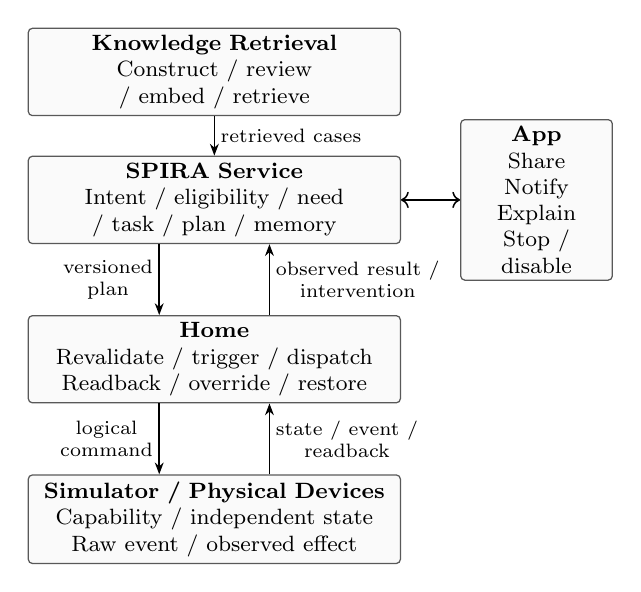
\begin{tikzpicture}[
  panel/.style={draw=black!65,fill=black!2,rounded corners=1.5pt,
    line width=0.45pt,align=center,font=\footnotesize,
    text width=4.55cm,inner sep=2.5pt},
  flow/.style={-{Stealth[length=1.5mm]},line width=0.55pt},
  exchange/.style={font=\scriptsize,align=center,inner sep=2pt}
]
\node[panel] (knowledge) {\textbf{Knowledge Retrieval}\\Construct / review / embed / retrieve};
\node[panel,below=5mm of knowledge] (service) {\textbf{SPIRA Service}\\Intent / eligibility / need / task / plan / memory};
\node[panel,text width=1.75cm,right=7.5mm of service] (app) {\textbf{App}\\Share\\Notify\\Explain\\Stop / disable};
\node[panel,below=9mm of service] (home) {\textbf{Home}\\Revalidate / trigger / dispatch\\Readback / override / restore};
\node[panel,below=9mm of home] (devices) {\textbf{Simulator / Physical Devices}\\Capability / independent state\\Raw event / observed effect};
\draw[flow] (knowledge) -- node[exchange,right] {retrieved cases} (service);
\draw[flow,<->] (service) -- (app);
\draw[flow] ([xshift=-7mm]service.south) -- node[exchange,left] {versioned\\plan} ([xshift=-7mm]home.north);
\draw[flow] ([xshift=7mm]home.north) -- node[exchange,right] {observed result /\\intervention} ([xshift=7mm]service.south);
\draw[flow] ([xshift=-7mm]home.south) -- node[exchange,left] {logical\\command} ([xshift=-7mm]devices.north);
\draw[flow] ([xshift=7mm]devices.north) -- node[exchange,right] {state / event /\\readback} ([xshift=7mm]home.south);
\end{tikzpicture}
\caption{Logical system flow and responsibility boundaries.}
\label{fig:logical-flow}
\end{figure}

Knowledge Retrieval prepares and returns synthetic purchase-intent cases. Service interprets intent, derives household needs, applies product policy, versions plans, prepares explanations, and updates memory. App handles order sharing, notification, explanation, and user controls. Home owns live capability and state checks, local triggers, command dispatch, readback, override handling, and restoration. A simulator or physical device keeps its own state and reports the result of a command. This responsibility map specifies behavior; deployment architecture belongs to Phase C.

\subsection{Choice of Software Development Platform}
Development uses a MacBook Air (\texttt{Mac16,12}) with an Apple M4 processor, 10 CPU cores, 16 GB of memory, and macOS 26.5 (build 25F71). It runs the Service, retrieval pipeline, database, simulator, and mobile-development tools on one machine, which keeps the prototype reproducible and allows direct testing over the home network. The Home prototype reuses a Galaxy S10 5G running Android 16, LineageOS 23.2, and Kali Rolling 2026.1. The phone provides local trigger processing, state checks, and device adapters without adding a Raspberry Pi.

Python 3.12 is used for retrieval, the Service, Home logic, and simulation because those components share model clients, validation code, HTTP handling, database access, and test utilities. The App uses Flutter 3.47.5 and its bundled Dart SDK so that order sharing, notifications, explanations, and controls can be maintained in one mobile codebase. PostgreSQL 16 with pgvector stores episode data and the synthetic-case index.

The local prototype reuses the MacBook Air, Galaxy S10 5G, Tapo C200, and available phones, so its incremental hardware cost is KRW 0. The selected open-source stack adds no licence fee. Synthetic-data generation and runtime model use are budgeted at KRW 30,000--35,000, below the KRW 50,000 project ceiling. Cloud service and new-device costs are excluded because the current prototype neither requires nor claims them.

\subsection{Software in Use}
The software baseline is Python 3.12.13, FastAPI 0.162.0, Uvicorn 0.54.0, PostgreSQL 16.15, pgvector 0.8.7, Docker Engine 29.5.2, Docker Compose 5.1.4, and Flutter 3.47.5 with its bundled Dart SDK. Docker Compose reproduces the local Service and database environment. FastAPI and Uvicorn expose the prototype's HTTP and JSON exchanges, while PostgreSQL keeps orders, decisions, plan versions, results, and household memory.

Knowledge Retrieval encodes accepted synthetic cases with the BGE-M3 embedding family \cite{ref15} and ranks them by vector similarity. A structured language-model call then produces one intent or no-intent judgment. The remaining control path is deterministic: schema checks validate model output, plan rules reject unsupported or prohibited effects, Home rechecks live state, and readback distinguishes command acceptance from an observed result. Python and database version policies are documented by their official projects \cite{ref9}--\cite{ref13}; Flutter installation and versioning follow the official manual \cite{ref14}.

\subsection{Task Distribution}
\begin{table}[H]
\caption{Task Distribution}
\centering
\footnotesize
\setlength{\tabcolsep}{2.5pt}
\renewcommand{\arraystretch}{1.08}
\begin{tabularx}{\columnwidth}{@{}>{\raggedright\arraybackslash}p{0.18\columnwidth}>{\raggedright\arraybackslash}p{0.18\columnwidth}>{\raggedright\arraybackslash}X@{}}
\toprule
\textbf{Role} & \textbf{Member} & \textbf{Task description} \\
\midrule
User & Uijin Lee & Tests order sharing, explanations, alerts, and controls; prepares and reviews synthetic purchase-intent cases \\
Customer & Seojin Lee & Defines objectives and scope, reviews the birthday and contrast scenarios, and checks requirement coverage \\
Software developer & Yejoon Kim & Implements model integration, Service and database behavior, event processing, device adapters, and tests \\
Development manager & Jeewon Lee & Manages the schedule, task allocation, meeting records, requirement traceability, and submission integration \\
\bottomrule
\end{tabularx}
\label{tab:auto-1}
\end{table}
\section{Specifications}
One episode proceeds through order intake, intent interpretation, plan formation, local execution, observation, and memory.

\subsection{Order Intake and Intent Interpretation}
Household setup begins with an authenticated user and a revocable Home credential. Home reports the effects needed by the birthday scenario, including value constraints, reversibility, availability, and current state. Service stores the report separately from product policy, so device support alone never permits execution.

Android receives an order selected by the user through \texttt{ACTION\_SEND}, while iOS uses a Share Extension. The App sends only the selected text or image, sharing consent, and a stable source identifier. A repeated identifier returns the existing episode. Service extracts visible item names, quantities, arrival information, product groups, and supported attributes; ambiguous values remain unknown. The source image is deleted after extraction, and sensitive item titles are generalized or removed before intent processing.

Intent context combines the structured order with relevant time or calendar tags and retrieved purchase-intent cases. Raw calendar text, unrelated history, current device state, capability catalogs, and household execution memory are excluded from the judgment. The result identifies a possible situation, its relevant item bundle, excluded items, unknown details, and supporting evidence. A valid no-intent result ends situation planning without error.

The synthetic corpus is produced in stages. The team reviews an initial set of about 100 complete cases for unsupported detail, duplication, sensitivity, and structural errors, corrects the generation process, and then expands toward 1,000 cases. Accepted cases retain synthetic status and review provenance before embedding. These counts describe the production sequence, not a runtime permission threshold.

\begin{figure}[!t]
\noindent\begin{minipage}{\columnwidth}
\begin{lstlisting}
interpret_order(shared_order, household):
    order = extract_visible_fields(shared_order)
    context = select_time_and_purchase_context(order)
    cases = retrieve_accepted_cases(order, context)
    decision = validate(infer_once(order, context, cases))
    if decision is invalid or sensitive:
        return close_without_preparation(reason)
    if decision is no_intent:
        return close_normally()
    return record_situation(decision, order, cases)
\end{lstlisting}
\end{minipage}
\end{figure}
Service checks the response structure, item references, and cited evidence. Similarity and confidence support explanation and offline evaluation; they do not authorize physical action. Household authorization, product policy, device eligibility, and user controls are evaluated after intent judgment.

\subsection{Need, Guidance, and Plan Formation}
Service states the household need before selecting a device effect. For example, "prepare a child-safe guest environment" may map to supported lighting, cleaning, and safety effects. If no registered capability can meet the need, the episode contains guidance or no task. Handling advice is added only when the situation changes normal handling, omission risks material loss, or a preparation step is not obvious. The birthday scenario therefore treats strawberries and cream differently from ordinary grocery storage while suppressing repeated advice.

Each task records its plan and task identifiers, plan version, target, desired effect, trigger, validity period, preconditions, temporary-state rule, and explanation. Before publication, Service checks the target, value range, time window, room and quiet-hour rules, and product policy. High-risk cooking and washing starts are prohibited; an oven task may prepare a safe standby setting, but a person starts cooking.

\noindent\begin{minipage}{\columnwidth}
\begin{lstlisting}
build_plan(situation, household):
    needs = derive_household_needs(situation)
    tasks = map_needs_to_registered_capabilities(needs)
    tasks += eligible_item_guidance(situation.items)
    for task in tasks:
        require valid_target_and_value(task)
        require valid_time_and_trigger(task)
        require product_policy_allows(task)
    resolve_conflicts(tasks)
    return publish_new_version(tasks)
\end{lstlisting}
\end{minipage}
A relevant calendar, capability, task, or user-control change creates a new immutable plan version. Home executes only the current version. Equivalent effects may be merged; incompatible effects on the same target and time interval are rejected with a visible reason. A superseded pending task cannot start a new effect, while work already dispatched keeps its actual result record.

\subsection{Local Execution and Recovery}
Execution runs at Home. It obtains the current plan over outbound HTTPS, evaluates package, schedule, arrival, event-end, and device triggers locally, and posts results to Service. Immediately before dispatch it rechecks the plan version, deadline, stop or disable state, live capability, physical state, human use, and recent manual changes. A disconnected Home does not start a new effect from a cached plan.

\begin{figure}[!t]
\noindent\begin{minipage}{\columnwidth}
\begin{lstlisting}
execute_task(task, event):
    plan, state = fetch_current_plan_and_state()
    if task is stale, stopped, disabled, expired, or ineligible:
        return not_started(reason)
    if desired_effect_already_holds(state):
        return verified_no_change()
    prior = capture_state_if_temporary(task)
    acceptance = dispatch_once(task)
    observed = read_back_effect()
    return record_result(acceptance, observed, prior)
\end{lstlisting}
\end{minipage}
\end{figure}
Home records command acceptance separately from observed effect. Readback produces verified, partial, failed, or unknown results; a timeout is not success. \texttt{STOP ALL} blocks later starts and requests best-effort cancellation of work already in flight. \texttt{DISABLE TASK} affects the selected task and any actual dependency. Stable episode, plan, task, and attempt identifiers make retries duplicate-safe.

Safety checks run during plan validation, pre-dispatch revalidation, and result handling. A manual or external change takes precedence and prevents immediate reassertion. Before a temporary effect, Home saves the prior state. Restoration occurs only when that state still exists, the effect is attributable to SPIRA, and no later user or external change has taken ownership. Local triggers do not wait for a public inbound connection, and uncertain outcomes are reconciled by later status or readback.

\subsection{Observation, Memory, and Interaction}
Service opens an observation window only for an active episode and retains evidence needed to evaluate its tasks. Each value is labeled as commanded, accepted, observed, inferred, simulated, or user-provided. SPIRA-generated effects are removed from the household baseline used to interpret later state. General indoor cameras, wearables, and per-item tracking are outside the prototype.

Household memory links the inferred situation, attempted work, observed result, explicit reaction, provenance, and physical or simulated path. Silence and a compatible device state do not establish satisfaction or future permission. A correction can influence later planning without model retraining. Revocation stops new use, and deletion removes the record from later retrieval and planning.

\noindent\begin{minipage}{\columnwidth}
\begin{lstlisting}
close_episode(episode):
    evidence = collect_permitted_observations(episode.window)
    memory = link(evidence, episode.situation,
                  episode.tasks, episode.explicit_reaction)
    if retention_is_allowed(memory) and
       useful_for_later_preparation(memory):
        store(memory)
    else:
        keep_episode_record_only()
\end{lstlisting}
\end{minipage}
The App uses one episode card showing the interpreted situation, planned preparation, short rationale, task status, and physical or simulated label. \texttt{WHY?} reads the stored decision and execution evidence without repeating inference. No-intent, zero-task, routine start, and routine completion remain quiet unless the user opens the episode. Screenshots, structured orders, intent decisions, execution evidence, and reusable memory have separate purposes and retention rules. External model requests contain the structured order, selected context, and retrieved cases, not unrelated household history.

\subsection{Evaluation and Demonstration}
The retrieval component is tested on held-out orders with the same model and context in two conditions: synthetic retrieval enabled and retrieval disabled. The comparison records intent or no-intent judgment, relevant-item selection, unsupported detail, and output validity. End-to-end traces separately record plan validity, command acceptance, observed effect, stop or override handling, restoration, and scenario completion.

The main demonstration is the birthday-party episode, accompanied by one ordinary or no-intent case and one override or restoration case. The simulator maintains device state independently, emits scripted doorbell, lock, camera, and user events, and supports a virtual clock for replaying the multi-day scenario during a short presentation. Every interface and result identifies whether the path is physical or simulated. An unavailable vendor interface is shown as simulated or unsupported.

\balance
\begin{thebibliography}{99}
\scriptsize
\bibitem{ref1}P. Sarantopoulos, A. Theotokis, K. Pramatari, and G. Doukidis, ``Shopping missions: An analytical method for the identification of shopper need states,'' \emph{Journal of Business Research}, vol. 69, no. 3, pp. 1043--1052, 2016, doi: \href{https://doi.org/10.1016/j.jbusres.2015.08.017}{10.1016/j.jbusres.2015.08.017}.
\bibitem{ref2}Z. Sun, J. Yang, K. Feng, H. Fang, X. Qu, and Y. S. Ong, ``Revisiting bundle recommendation: Datasets, tasks, challenges and opportunities for intent-aware product bundling,'' in \emph{Proceedings of the 45th International ACM SIGIR Conference on Research and Development in Information Retrieval}, 2022, pp. 2900--2911, doi: \href{https://doi.org/10.1145/3477495.3531904}{10.1145/3477495.3531904}.
\bibitem{ref3}Z. Sun, K. Feng, J. Yang, X. Qu, H. Fang, Y.-S. Ong, and W. Liu, ``Adaptive in-context learning with large language models for bundle generation,'' in \emph{Proceedings of the 47th International ACM SIGIR Conference on Research and Development in Information Retrieval}, 2024, pp. 966--976, doi: \href{https://doi.org/10.1145/3626772.3657808}{10.1145/3626772.3657808}.
\bibitem{ref4}C. Yu, X. Liu, J. Maia, T. Cao, L. Li, Y. Gao, Y. Song, R. Goutam, H. Zhang, B. Yin, and Z. Li, ``COSMO: A large-scale e-commerce common sense knowledge generation and serving system at Amazon,'' in \emph{Companion Proceedings of the 2024 International Conference on Management of Data}, 2024, doi: \href{https://doi.org/10.1145/3626246.3653398}{10.1145/3626246.3653398}.
\bibitem{ref5}S. Zeng, J. Zhang, P. He, J. Ren, T. Zheng, H. Lu, H. Xu, H. Liu, Y. Xing, and J. Tang, ``Mitigating the privacy issues in retrieval-augmented generation via pure synthetic data,'' in \emph{Proceedings of the 2025 Conference on Empirical Methods in Natural Language Processing}, 2025, pp. 24527--24558, doi: \href{https://doi.org/10.18653/v1/2025.emnlp-main.1247}{10.18653/v1/2025.emnlp-main.1247}.
\bibitem{ref6}A. Salemi, S. Mysore, M. Bendersky, and H. Zamani, ``LaMP: When large language models meet personalization,'' in \emph{Proceedings of the 62nd Annual Meeting of the Association for Computational Linguistics, Volume 1: Long Papers}, 2024, pp. 7370--7392, doi: \href{https://doi.org/10.18653/v1/2024.acl-long.399}{10.18653/v1/2024.acl-long.399}.
\bibitem{ref7}E. King, H. Yu, S. Lee, and C. Julien, ``Sasha: Creative goal-oriented reasoning in smart homes with large language models,'' \emph{Proceedings of the ACM on Interactive, Mobile, Wearable and Ubiquitous Technologies}, vol. 8, no. 1, article 12, pp. 1--38, 2024, doi: \href{https://doi.org/10.1145/3643505}{10.1145/3643505}.
\bibitem{ref8}S. Li, Y. Guo, J. Yao, Z. Liu, and H. Wang, ``HomeBench: Evaluating LLMs in smart homes with valid and invalid instructions across single and multiple devices,'' in \emph{Proceedings of the 63rd Annual Meeting of the Association for Computational Linguistics, Volume 1: Long Papers}, 2025, pp. 12230--12250, doi: \href{https://doi.org/10.18653/v1/2025.acl-long.597}{10.18653/v1/2025.acl-long.597}.
\bibitem{ref9}Python Software Foundation, ``Status of Python versions.'' [Online]. Available: https://devguide.python.org/versions/.
\bibitem{ref10}FastAPI, ``fastapi 0.162.0.'' \emph{Python Package Index}. [Online]. Available: https://pypi.org/project/fastapi/0.162.0/.
\bibitem{ref11}M. Trylesinski and contributors, ``uvicorn 0.54.0.'' \emph{Python Package Index}. [Online]. Available: https://pypi.org/project/uvicorn/0.54.0/.
\bibitem{ref12}PostgreSQL Global Development Group, ``PostgreSQL versioning policy.'' [Online]. Available: https://www.postgresql.org/support/versioning/.
\bibitem{ref13}pgvector contributors, ``pgvector changelog.'' [Online]. Available: https://github.com/pgvector/pgvector/blob/master/CHANGELOG.md.
\bibitem{ref14}Flutter, ``Install Flutter manually.'' [Online]. Available: https://docs.flutter.dev/install/manual.
\bibitem{ref15}J. Chen, S. Xiao, P. Zhang, K. Luo, D. Lian, and Z. Liu, ``BGE M3-embedding: Multi-lingual, multi-functionality, multi-granularity text embeddings through self-knowledge distillation,'' arXiv:2402.03216, 2024.
\end{thebibliography}
\end{document}
